\chapter{Coupled CFD-DEM Models Revealing the Influence of Helium Purge Gas on Effective Thermal Conductivity of a Pebble Bed Experiencing Pebble Crushing}\label{sec:cfd-dem-studies}
The numerical implementation of fluid-solid interaction was outline in \cref{sec:modeling-cfd-dem}. Although we are most interested in the thermal response of the packed beds to the interestitial gas, we will begin by comparing the results of momentum interaction.
\subsection{Modeling Setup and Procedure}
The pebble bed has dimensions in the x-y directions of 20d×15d, respectively. There are structural walls, providing cooling, at the x-limits and periodic walls in the y-limits. 10 000 pebbles were loaded into the system which went to a height of approximately 24d after the bed was vibration packed. The pebble bed had a roof loaded at the upper limit of the z-direction that was lowered by force-control up to 6 MPa. This bed is referred to as the ‘well-packed’ bed. This was meant to simulate a fresh, densely-packed bed that is under compressive load during fusion operation. As such, this would be when pebbles would be likely to crack during operation. Therefore, based on the well-packed bed, a second bed was generated by simulating crushed pebbles; crudely the extensive crushing is simulated by simply removing 10\% of the pebbles at random from the ensemble and then allowing the bed to resettle, from the now-imbalanced gravity and inter-particle forces, to a new stable packing structure. This bed is then referred to as the ‘resettled’ bed for the rest of the analysis. The intent is to deduce changes in thermo-mechanical properties from an ideally packed bed to one where significant cracking has altered the ideal morphology of the bed. 
\section{Pressure Drop}
Before analyzing thermal results from the CFD-DEM coupling, the system was run at various particle Reynolds numbers and the overall pressure drop of the packed bed was measured. This value was compared against the well-known Kozeny-Carman and Ergun equations. The Kozeny-Carman is known to fit better with experimental data at very small Reynolds numbers. In Fig.~\ref{fig:cfdem-pressure-drop} we see the CFD-DEM coupling model is providing bed-scale pressure drops that match very well with Kozeny-Carman over the Reynold’s numbers applicable to helium purge flow in fusion reactors.

The flow is visualized in Fig.~\ref{fig:cfdem-streamlines}. The pebble bed is clipped at the centerline to allow viewing of the helium streamlines. Apparent in the figure is temperature profiles in the helium from centerline to wall that qualitatively mirror temperature profiles in the pebble bed.

\begin{figure}
        \centering
        \begin{subfigure}[b]{0.7\textwidth}
                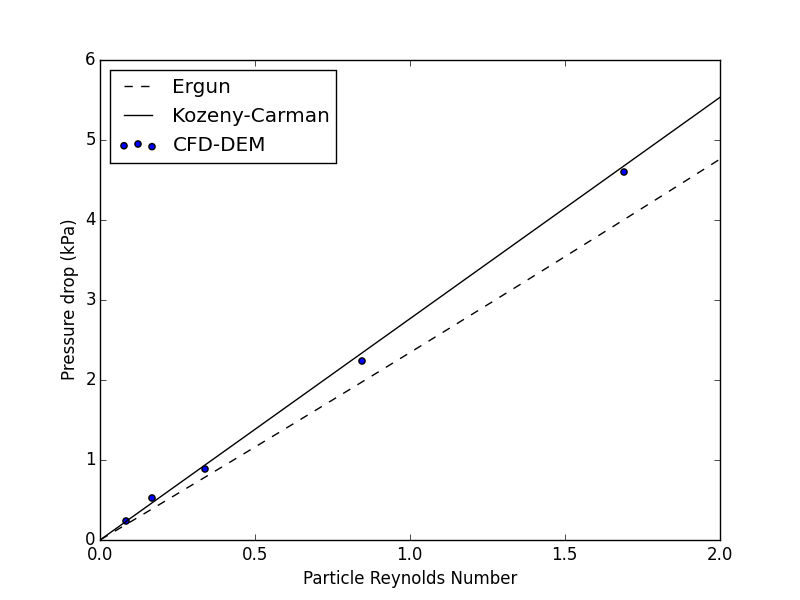
\includegraphics[width=\textwidth]{chapters/figures/pressureDrops-full.png}
                \caption{Well-packed bed}
                \label{fig:pressure-drop-full}
        \end{subfigure}%
        
          %add desired spacing between images, e. g. ~, \quad, \qquad, \hfill etc.
          %(or a blank line to force the subfigure onto a new line)
        \begin{subfigure}[b]{0.7\textwidth}
                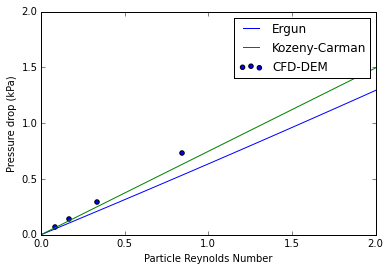
\includegraphics[width=\textwidth]{chapters/figures/pressureDrops-evap.png}
                \caption{Re-settled bed}
                \label{fig:pressure-drop-evap}
        \end{subfigure}
        \caption{Pressure drop calculations across packed beds, solved by CFD-DEM, fit well to the Kozeny-Carman empirical relation.}\label{fig:cfdem-pressure-drop}
\end{figure}



\begin{figure}[t]
	\centering
	\caption{Cut-away view of the pebble bed with streamlines of helium moving in generally straight paths from inlet to exit.}
	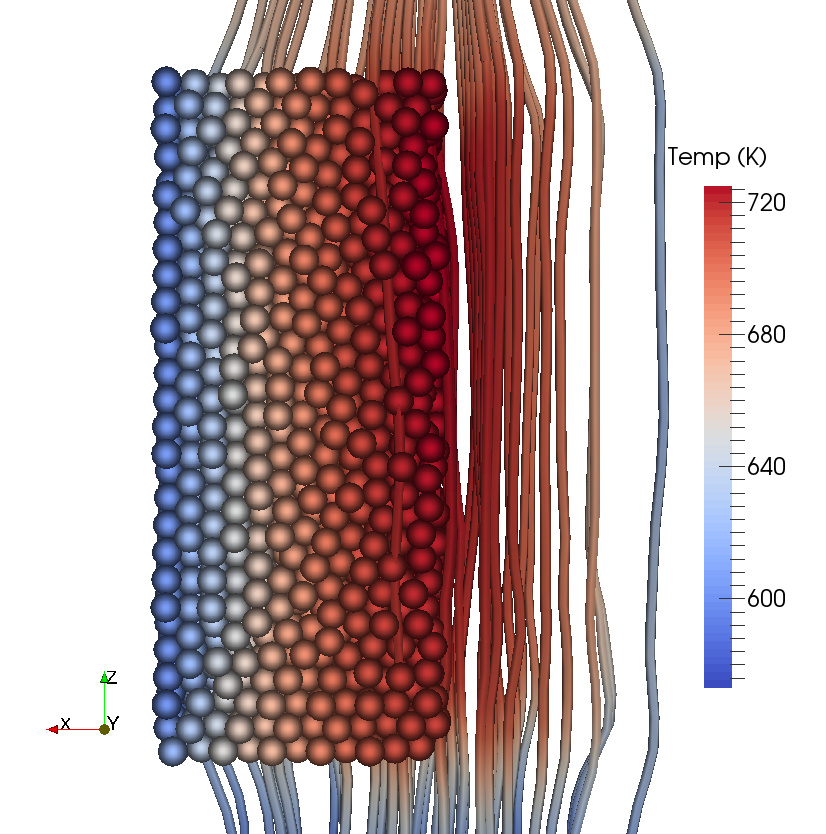
\includegraphics[width=0.75\textwidth]{chapters/figures/cfd-dem-streamlines2}\label{fig:cfdem-streamlines}
\end{figure}




\begin{figure}
        \centering
        \begin{subfigure}[b]{0.5\textwidth}
                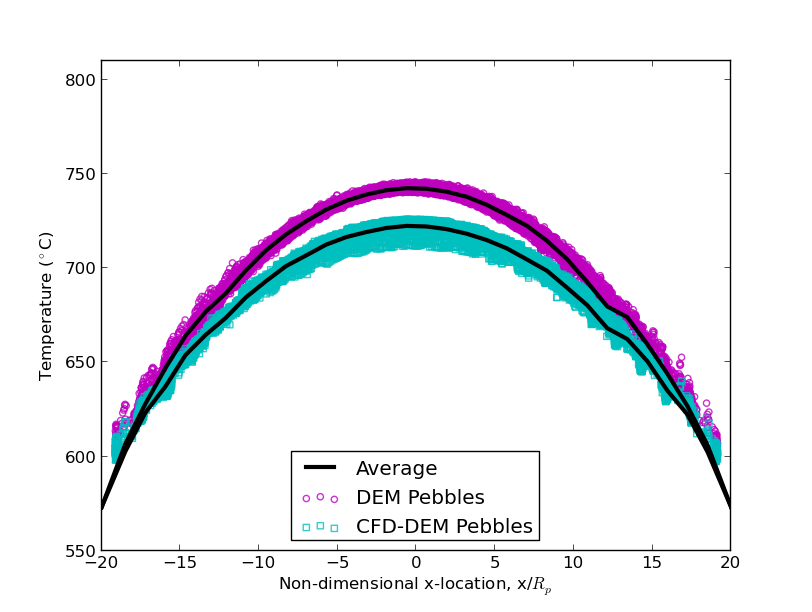
\includegraphics[width=\textwidth]{chapters/figures/full-x-T-color}
                \caption{Well-packed bed}
                \label{fig:x-T-full}
        \end{subfigure}%
        
          %add desired spacing between images, e. g. ~, \quad, \qquad, \hfill etc.
          %(or a blank line to force the subfigure onto a new line)
        \begin{subfigure}[b]{0.5\textwidth}
                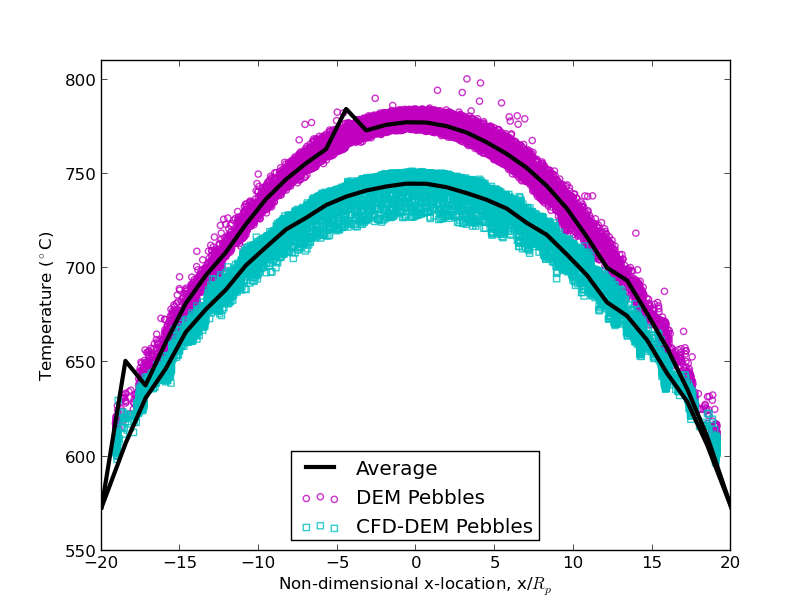
\includegraphics[width=\textwidth]{chapters/figures/evap-x-T-color}
                \caption{Re-settled bed}
                \label{fig:x-T-evap}
        \end{subfigure}
        \caption{Scatter temperature profiles of pebbles in a bed that is: well-packed (left) and resettled after 10\% of pebbles were removed from crushing (right). The introduction of helium into the simulation contributes to both lower overall temperatures (higher effective conductivity) and the smoothing out of high temperatures of isolated pebbles.}\label{fig:cfdem-x-T}
\end{figure}
\subsection{Effective Thermal Conductivity from CFD-DEM}\label{sec:cfd-dem-effective-conductivity}

The simulation is allowed to run to thermal steady-state with nuclear heating and wall cooling. After reaching a steady solution, I analyze the temperature profiles of the fluid and pebble bed. The temperature of the fluid volume from the simulation of the well-packed bed is shown in Fig.~\ref{fig:cfdem-complete-domain}. The flow field is also visualized in Fig.~\ref{fig:cfdem-streamlines}; in this figure the pebble bed is clipped at the centerline to allow viewing of the helium streamlines. Apparent in the figure is temperature profiles in the helium from centerline to wall that qualitatively mirror temperature profiles in the pebble bed. The two beds in our system, well-packed and resettled, were run to thermal steady-state with nuclear heating and wall cooling in both pure DEM and coupled CFD-DEM simulations for comparison. From steady-state temperature distributions, seen in the pebble scatter plots in Fig.~\ref{fig:cfdem-x-T}, an average profile is calculated and an effective thermal conductivity computed following the procedure shown in \cref{sec:keff-analogy}. The values are tabulated in Table~\ref{tab:cfdem-keff}. 

In the case of pure DEM, energy is transported solely along conduction routes in the ensemble. When the packing of the bed is disturbed, this results in a substantial drop in effective conductivity (a drop of 31\%). Perhaps more important than the reduction in effective conductivity, is the growth in number of isolated rattlers. Because heat deposition is volumetrically applied, pebbles with poor conduction routes become much hotter than their neighbors. This is evident in the high temperatures seen in many of the pebbles in the Fig.~\ref{fig:x-T-evap}. Over-heating of isolated pebbles could induce sintering and impact their tritium release even when the average temperatures measured in the bed are well below sintering values.

When CFD-DEM beds are analyzed, there is still a large reduction in effective conductivity (22\% drop), but interesting to note is the lack of high temperature rattlers. In the CFD-DEM scatter plot of Fig.~\ref{fig:x-T-evap}, there is evidence of the reduced heat transfer in the same region as the isolated pebbles from the DEM bed, but the temperatures are much closer to the average values of neighboring pebbles. The helium purge gas has locally smoothed out the temperatures and provided heat transport paths for pebbles that have loose physical contact with neighbors.

In spite of the 22\% decrease in effective conductivity, the maximum temperature of the pebble bed only increased 6.2\% (from \SIlist{725;751}{\kelvin} when helium is included in the model. This result is significant for solid breeder designers. They may choose a solid breeder volume such that in the event of extensive pebble cracking, the maximum temperature of the bed would remain within the ideal windows dictate for the lithium ceramics.

An accompanying result is the increased amount of energy carried out of the system by the helium purge gas. In Table I, the last column provides the ratio of energy carried out of the system to the nuclear energy deposited into the bed. The amount of energy carried out by the helium increased from \numlist{1.15;1.52}\% from the well-packed to damaged beds.

\begin{figure}[t]
    \centering
    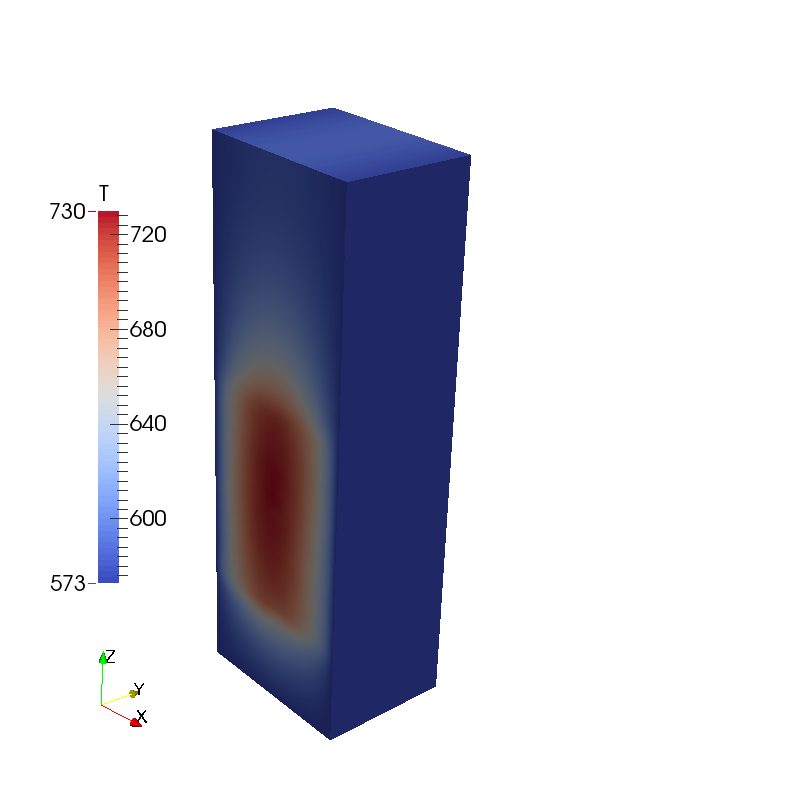
\includegraphics[width=\singleimagewidth]{chapters/figures/full-cfd-dem-fluid-temp}
    \caption{View of the complete fluid domain at thermal steady state.}\label{fig:cfdem-complete-domain}
\end{figure}


\begin{figure}[t]
    \centering
    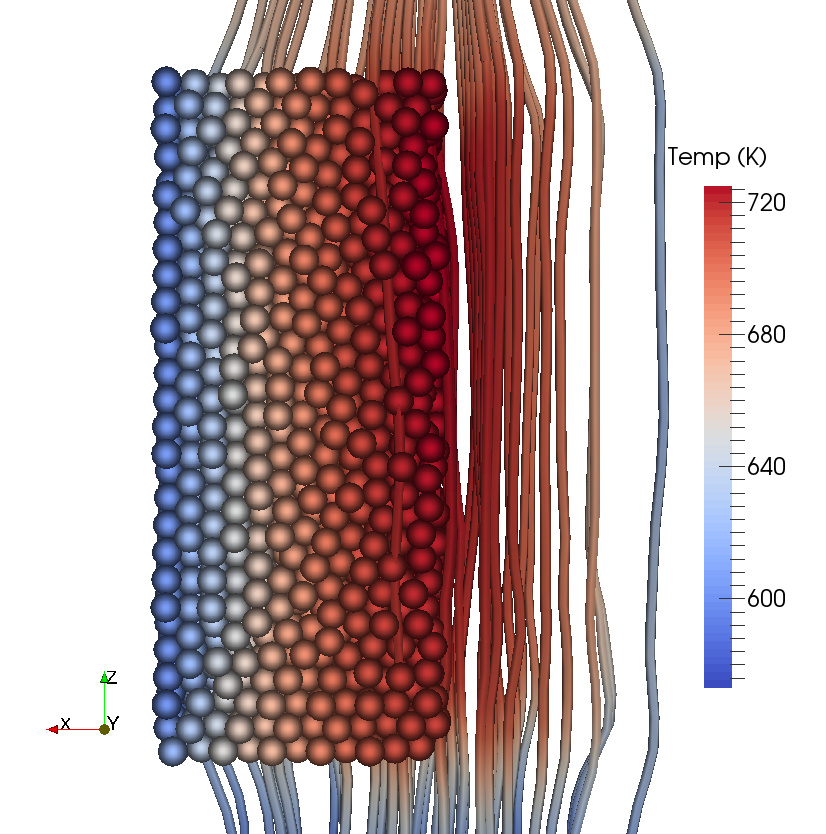
\includegraphics[width=\singleimagewidth]{chapters/figures/cfd-dem-streamlines2}
    \caption{Cut-away view of the pebble bed with streamlines of helium moving in generally straight paths from inlet to exit.}\label{fig:cfdem-streamlines}
\end{figure}


\begin{figure}
        \centering
        \begin{subfigure}[b]{0.5\textwidth}
                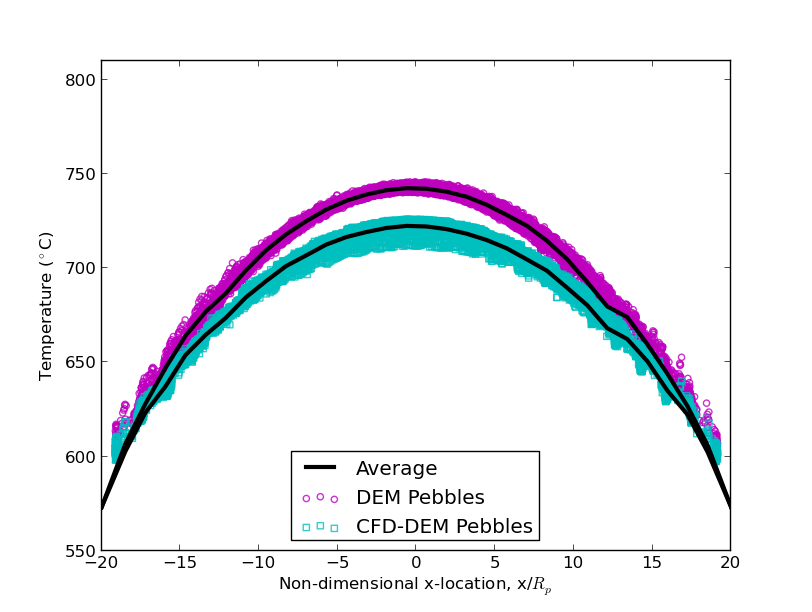
\includegraphics[width=\textwidth]{chapters/figures/full-x-T-color}
                \caption{Well-packed bed}
                \label{fig:x-T-full}
        \end{subfigure}%
        
          %add desired spacing between images, e. g. ~, \quad, \qquad, \hfill etc.
          %(or a blank line to force the subfigure onto a new line)
        \begin{subfigure}[b]{0.5\textwidth}
                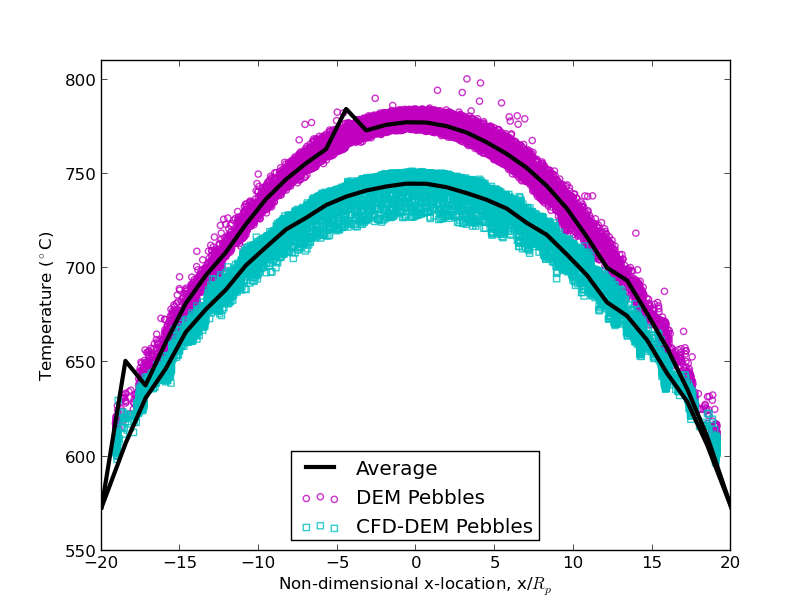
\includegraphics[width=\textwidth]{chapters/figures/evap-x-T-color}
                \caption{Re-settled bed}
                \label{fig:x-T-evap}
        \end{subfigure}
        \caption{Scatter temperature profiles of pebbles in a bed that is: well-packed (left) and resettled after 10\% of pebbles were removed from crushing (right). The introduction of helium into the simulation contributes to both lower overall temperatures (higher effective conductivity) and the smoothing out of high temperatures of isolated pebbles.}\label{fig:cfdem-x-T}
\end{figure}



\begin {table}[htp] %
\caption{Pebble bed values from the test matrix of the beds analyzed in this study.}
\label {tab:cfdem-keff} \centering %
\begin {tabular}{ rccccc }
\toprule %
			& 	\multicolumn{2}{c}{$\keff$}	&   \multicolumn{2}{c}{$T_\text{max}$}	&	$\frac{Q_h}{Q_\text{nuc}}$		\\
			& 	\multicolumn{2}{c}{(\si{\watt\per\meter\per\kelvin})}			&	\multicolumn{2}{c}{(\si{\kelvin})}				&									\\
			& 	DEM 		& 	CFD-DEM				&	DEM 		& 	CFD-DEM 			& 	CFD-DEM							\\\toprule
Well-packed	& 	0.96		& 	1.09				& 	745			& 	725					& 	1.15							\\
Resettled	& 	0.66		& 	0.85				& 	800			& 	751					& 	1.52							\\\bottomrule
\end{tabular}
\end{table}





\FloatBarrier


The CFD-DEM formulation maintains calculations of pebble-pebble interactions while dynamically coupling to the helium flow. The model demonstrates the ability of helium gas to smooth out any hot spots predicted by pure-conduction DEM formulations. Further, the lattice-Boltzmann simulation, while not fully coupled to DEM, revealed important features of helium flow in volumetrically heated pebble beds – mainly the smearing of temperature profiles along the paths of cooling.